\documentclass{article}
\usepackage{fancyhdr}
\usepackage[a4paper]{geometry}
\usepackage[colorlinks]{hyperref}
\usepackage{caption}
\usepackage{graphicx}
\usepackage[style=iso-numeric,alldates=iso,seconds=true]{biblatex}
\usepackage{tikz}
\usepackage{amsmath}
\usepackage{pgf-pie}
\usepackage{pgfplots}
\pgfplotsset{compat=1.18}
\addbibresource{ref.bib}
\title{The Overview of Transgender Community\\on the Internet in Mainland China}
\author{Seppei Chen}
\date{\today}
\pagestyle{fancy}
\fancyhead[RO]{\thepage}
\fancyhead[LO]{\bfseries The Overview of Transgender Community on the Internet of Mainland China}
\fancyfoot{}
\begin{document}
	\maketitle
	
	\begin{abstract}
		This study provides an exploratory overview of transgender community in Mainland China, a population of 4 million, but lack of understanding in the public. Combined with previous studies, statistics compiled by the author, news reports, and responses from the questionnaire made by the author. Demonstrated the factors controlling gender identity developments, medical resources for transgender people, and distributions across age, education, and region. Addressed the challenges that transgender people in Mainland China face, including family acceptance, accessibility to medical resources, legal restrictions, mental health crisis, and employment discrimination. Finally, the study explores the Internet platforms transgender people use, community subcultures, and the methods by which they are coping with challenges. Given its reliance on convenience sampling, the author emphasizes that this study could not be generalized to the whole transgender community, and wishes that further study could cover more transgender individuals for more accurate information.

        \textbf{Keywords:} online community; Mainland China; gender identity; LGBT discrimination
	\end{abstract}

	\section{Introduction}
	In conservative estimates, the transgender population in Mainland China is approximately 4 million people. Although many predecessors have performed studies about them, the majority still understand very little about such sexual minority communities. This study, as expected, aims to demonstrate situations within the transgender community in Mainland China. 

		\subsection{Method}
		This study employs the following research methods:
		\begin{itemize}
			\item Combining reports from previous study;
			\item Analysis of statistics compiled by the author before the project formally started as additional information;
			\item Referencing previous news reports from media.
			\item Making a questionnaire for surveying the Internet platforms that respondents use.\ (convenience sampling)
		\end{itemize}

	\section{What makes them become transgender}
	The reasons for letting them become transgender people are various. Generally, it is because of a combination of biological, psychological, and social factors that causes them to start to think their gender identity may not actually match their sex. Usually, the thought will be developed into gender dysphoria, and they will start to find medical resources to start the transition. If there is no additional problem, gender-affirming surgery (GAS) will be the last step for them to achieve the objective.

	\section{The medical resources}
		\subsection{Transgender women (TW)}
		The most commonly used medicines are estradiol (E2, usually in gel) and estradiol valerate (EV, usually in oral tablets, as shown in Figure~\ref{med:progynova}), and for some TW who can obtain drugs from the gray area, EV injectable (as shown in Figure~\ref{med:progynon}) is also a common hormone therapy medicine.

		\begin{figure}[t]
			\centering
			\begin{minipage}{0.45\linewidth}
				\centering
				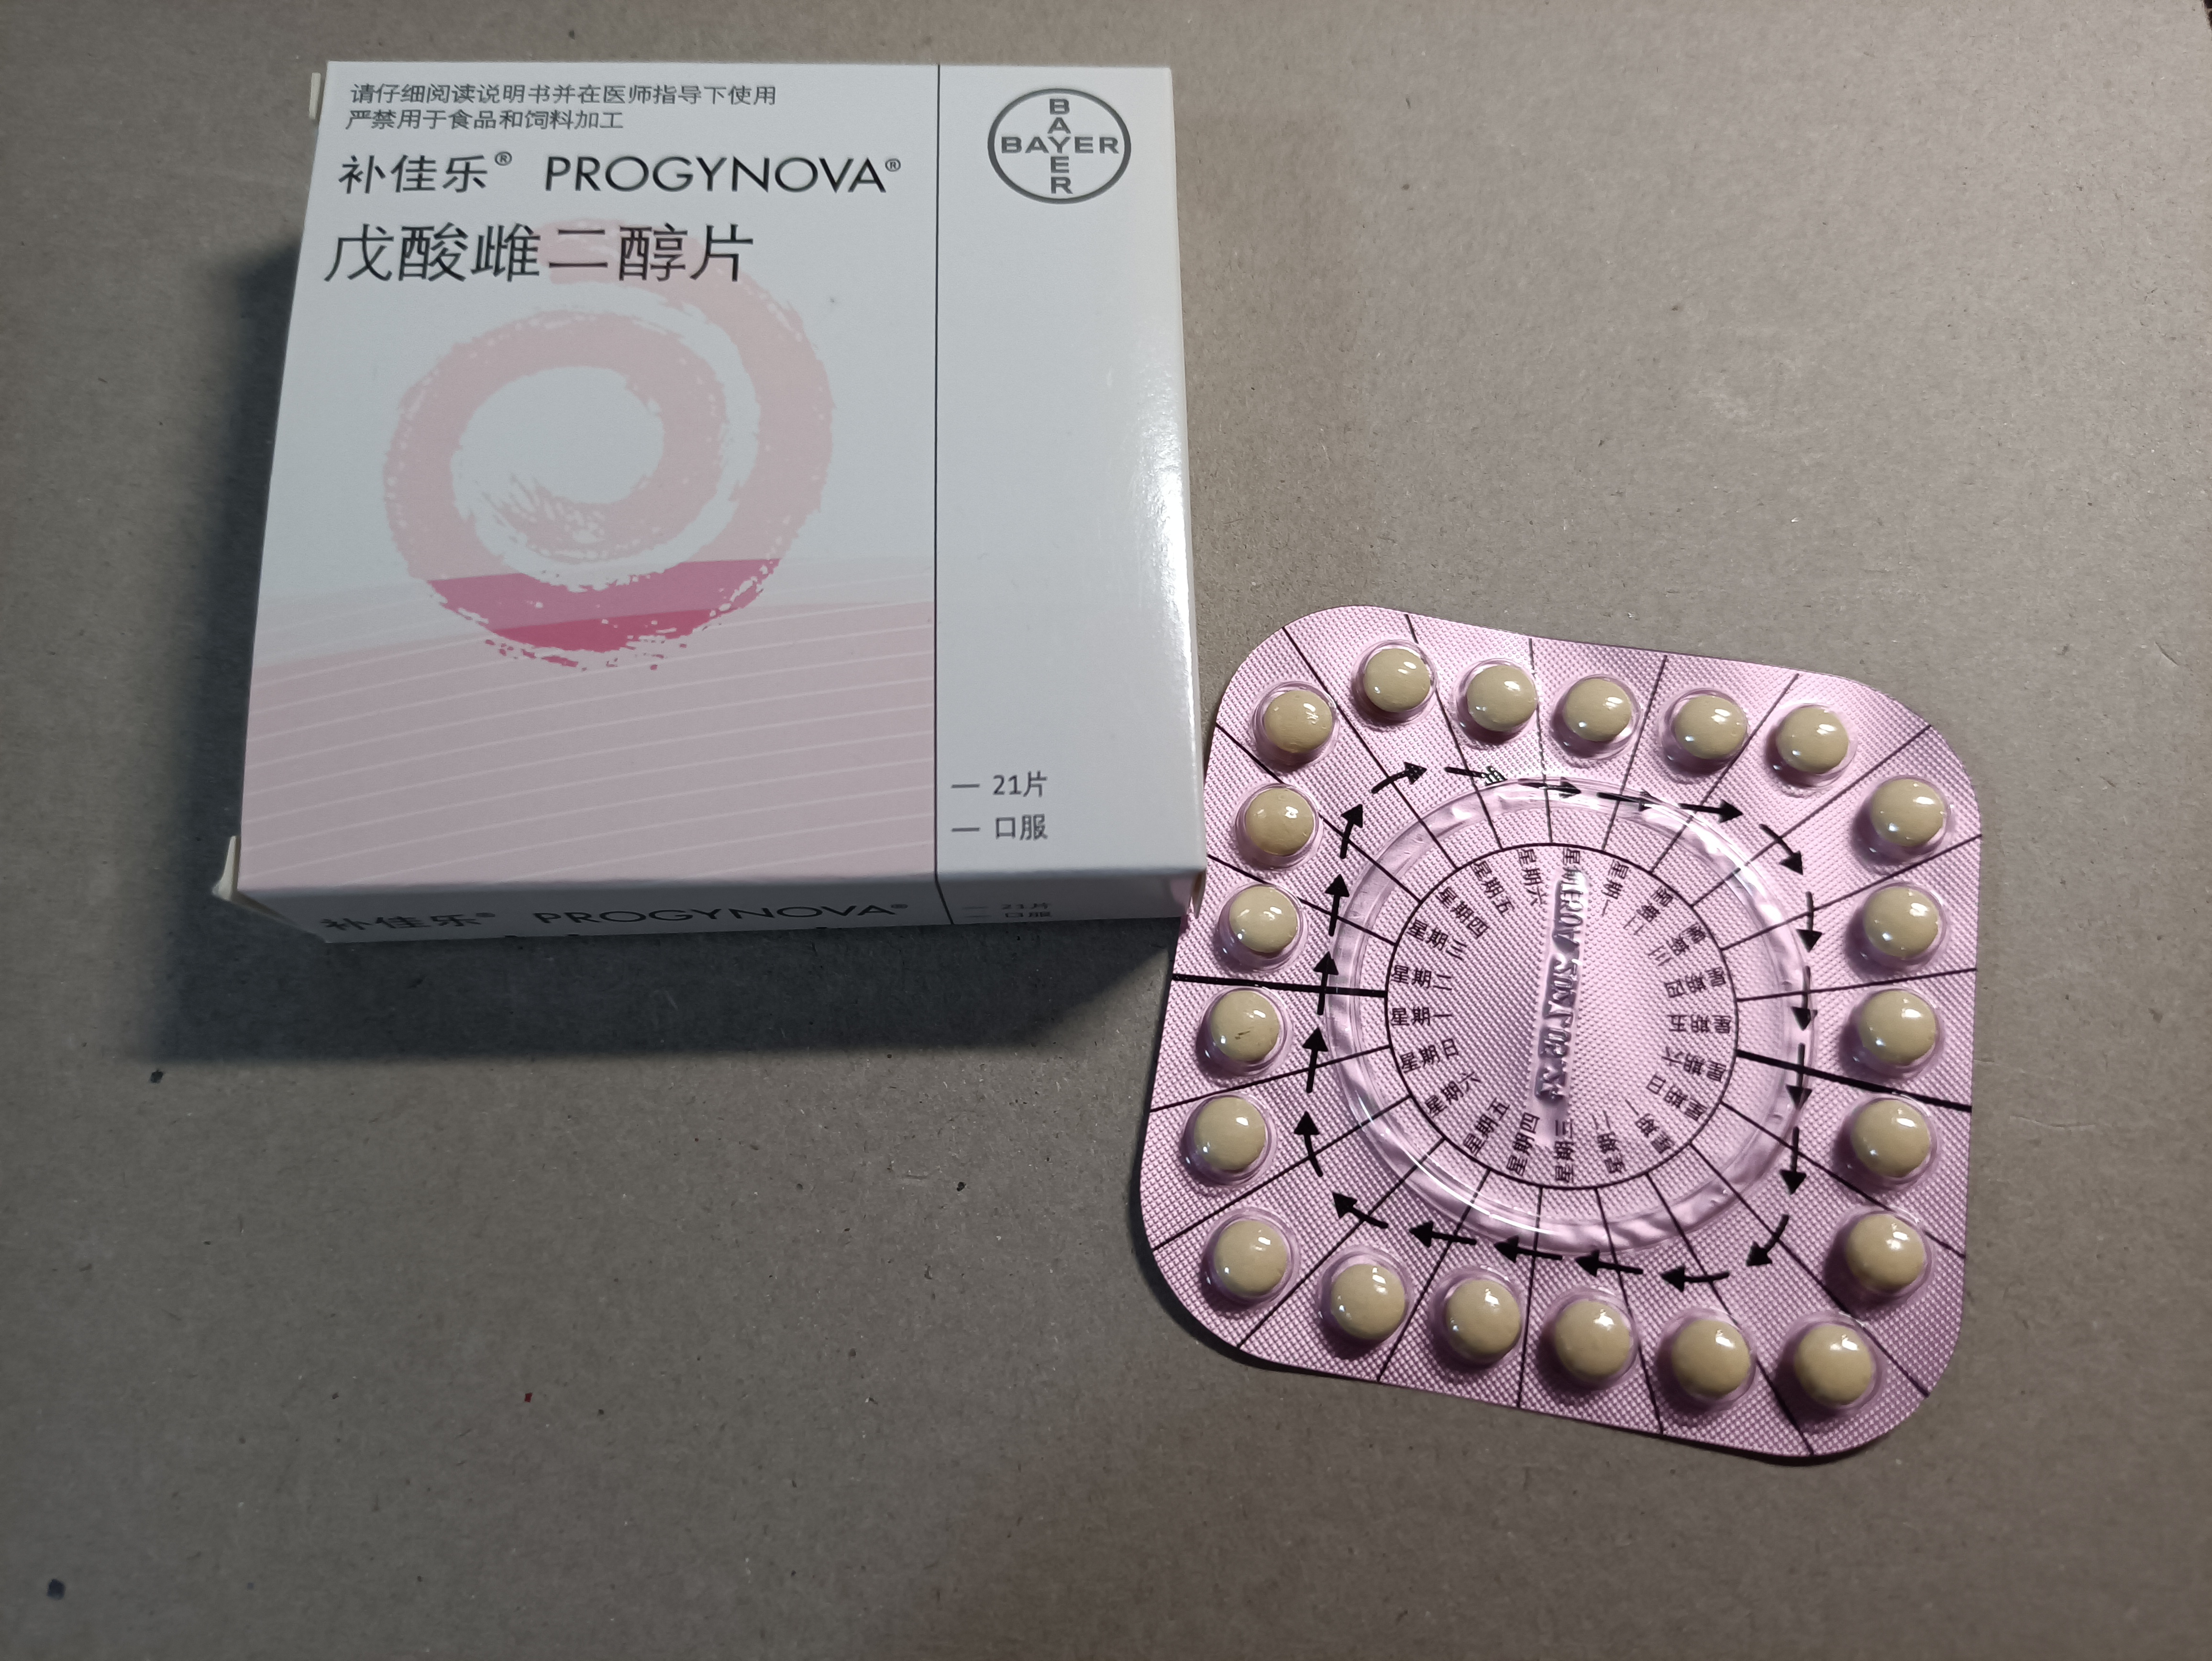
\includegraphics[height=3cm]{images/Progynova.jpg}
				\caption{Progynova (EV) 1 mg oral tablets in Mainland China}\label{med:progynova}
			\end{minipage}
			\qquad
			\begin{minipage}{0.45\linewidth}
				\centering
				
\includegraphics[height=3cm]{images/progynon-depot.jpg}
				\caption{Progynon-Depot (EV) 10 mg intramuscular injectable in Japan}\label{med:progynon}
				\end{minipage}
		\end{figure}

		Before starting to take estrogen, they need to take anti-androgen medicine first; usually, Androcur (as shown in Figure~\ref{med:anti}) is the most common choice.

		\subsection{Transgender men (TM)}
		For TM, testosterone undecanoate (TU, usually in injectables, as shown in Figure~\ref{med:TU}) is the most commonly used medicine for administering androgen. Other androgen medicines, due to their shorter half-life and the health risks to the body, are not recommended by the community.

		\begin{figure}[t]
			\centering
			\begin{minipage}{0.45\linewidth}
				\centering 
				
\includegraphics[height=3cm]{images/androcur.jpg}
				\caption{Androcur (cyproterone acetate) 50 mg oral tablets}\label{med:anti}
			\end{minipage}
			\qquad
			\begin{minipage}{0.45\linewidth}
				\centering
				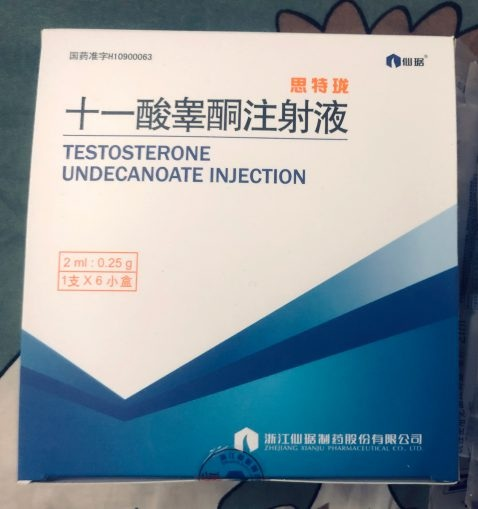
\includegraphics[height=3cm]{images/androgen.jpg}
				\caption{Testosterone undecanoate 250 mg intramuscular injectable in Mainland China}\label{med:TU}
			\end{minipage}
		\end{figure}

		Usually, anti-estrogen medicines are not needed. It is different from TW\@.

	\section{The distributions}
	According to a survey with 4296 samples by Jiayu Hou et al.~\cite{Hou_2026}, the median age of transgender people in Mainland China is 21; most of them have an undergraduate degree (\(59.4\%\)), and the runner-up is a high school degree (\(26.0\%\)) (as shown in Figure~\ref{dis:education}). Because of the survivor bias, students in high school are more likely to be seen on the Internet, and the trend is more significant at X (formerly Twitter). About the regional distribution, as stated by the same research, approximately \(60\%\) of transgender people live in big cities\footnote{Beijing, Shanghai, Shenzhen, and other provincial capitals in Mainland China, the same below.} (as shown in Figure~\ref{dis:residence}).

	\begin{figure}[hbp]
		\centering
		\begin{minipage}{0.45\linewidth}
			\centering
			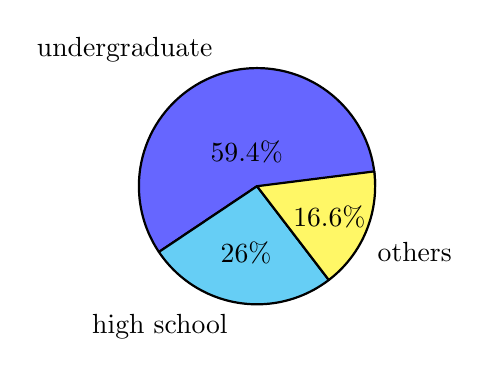
\begin{tikzpicture}[scale=0.5]
				\pie{59.4/undergraduate, 26/high school, 16.6/others}
			\end{tikzpicture}
			\caption{The distribution of respondents' education background}\label{dis:education}
		\end{minipage}
		\qquad
		\begin{minipage}{0.45\linewidth}
			\centering
			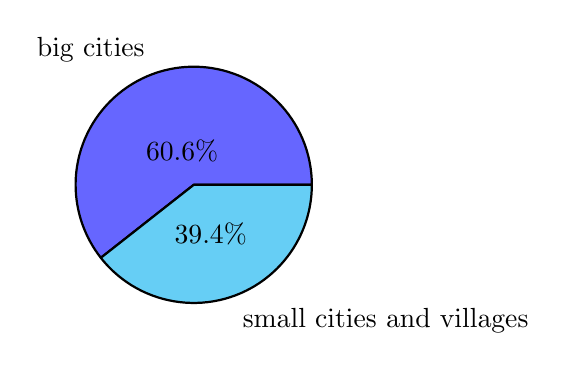
\begin{tikzpicture}[scale=0.5]
				\pie{60.6/big cities, 39.4/small cities and villages}
			\end{tikzpicture}
			\caption{The distribution of respondents' residences}\label{dis:residence}
		\end{minipage}
	\end{figure}

	\section{The challenges}
	Most transgender people in Mainland China lack support. And there are various factors that significantly increase the risk to their survival.
		\subsection{Low acceptance from the family}
		In line with traditional Chinese philosophy, the atmosphere in Mainland China is conservative. As noted in a 2017 report~\cite{Wu2017}, acceptance from family members is low (as shown in Figure~\ref{dis:accept}) among transgender people living in Mainland China.

		\begin{figure}[htp]
			\centering
			\begin{minipage}{0.8\linewidth}
				\centering
				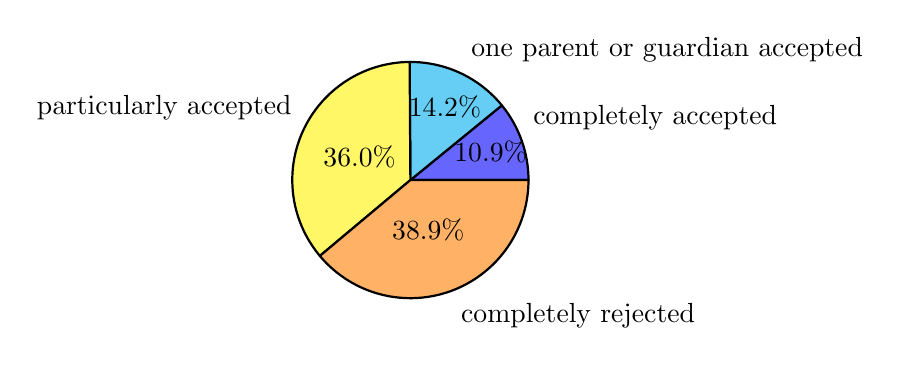
\begin{tikzpicture}[scale=0.5]
					\pie{10.9/completely accepted, 14.2/one parent or guardian accepted, 36.0/particularly accepted, 38.9/completely rejected}
				\end{tikzpicture}
				\caption{Level of gender identity acceptance: parents and guardians}\label{dis:accept}
			\end{minipage}
		\end{figure}

		As a result, coming out in the family is a dangerous decision for transgender people, especially for children without financial independence.

		Another thing that needs to be considered is the special educational organizations, which are illegal prisons by nature. The administrators of these schools will catch the anxiety from parents who find it hard to communicate with their child and the need to adjust behavioral deviations in the child, then promote advertisements to the public, and the parents who have seen the promotion will ask for help. Children, after experiencing abuse from the school, may behave ``normally''; however, they have been triggered, having little ability to return to their normal social life.

		\subsection{Difficult medical resources accessibility}
		In Mainland China, a prescription from the hospital is necessary for getting medicine from legal sources. However, the prescription is hard to get, especially for people who do not live in or near big cities. Even after getting the prescription, the medicine is also not easy to find in local pharmacies. So, transgender people in Mainland China tend to buy medicines via the Internet.

		However, in November 2022, the Chinese government announced a new policy~\cite{Gov2022}, which banned some particular medicines from online selling; drugs containing estradiol and cyproterone are clearly noted as ``banned''. Medicines containing testosterone are not directly mentioned, but are also affected by the ban on injectables.

		\subsection{Strict legal barrier}
		Nowadays, if a transgender person wants to change his or her mark on identity documents in Mainland China, he or she has to finish GAS first. But there are not many hospitals that have the ability to perform such surgeries. For that reason, many transgender people prefer to receive the operation in Thailand, which has better technological resources. However, the money needed is not easy for patients and their families to afford.

		In the post-op stage, there are still many real-life problems for transgender people. First, all the personal information related to the old identity will become invalid. They have to file a ticket at a police station to prove that both the old and new identity documents belong to the same person. On the other hand, at universities, once they graduate, all opportunities for changing information will be lost. That means they will not have an educational background, which may increase the difficulty of finding a job.

		\subsection{Mental health crisis}\label{sec:crisis}
		Mental health issues are always a serious problem in Mainland China, and this problem is more significant among transgender people. As research published in 2019 reported~\cite{Chen_2019}, approximately \(55.9\%\) (\(732 \div 1309 \times 100\%\)) of them are showing suicidal ideation, and \(28.4\%\) (\(209 \div 732 \times 100\%\)) of them have attempted to commit suicide, while these numbers are \(23.79\%\) (\(19145 \div 80489 \times 100\%\)) and \(7.5\%\) (\(1430 \div 19145 \times 100\%\)) among general population~\cite{Sun_2023}. According to a longitudinal dataset compiled by the author from publicly available posts on X (formerly Twitter) before this study (as shown in Figure~\ref{dis:suicide}), reports of suicide cases involving transgender individuals in Mainland China appear to be most frequent from late winter through early spring.

		\begin{figure}[htbp]
			\centering
			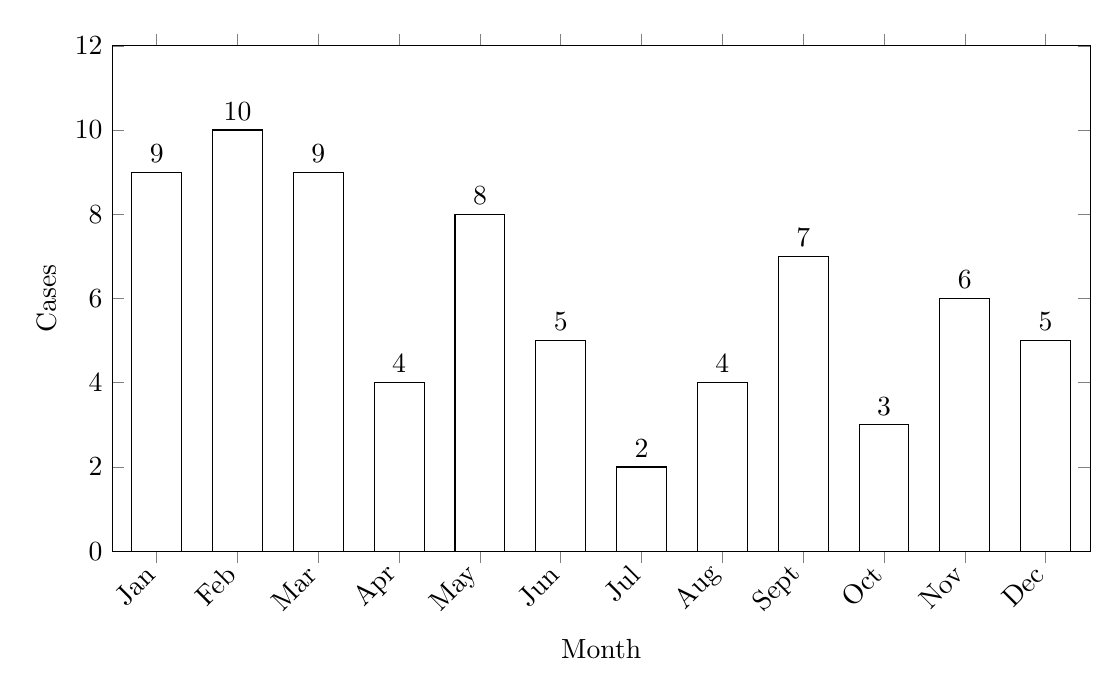
\begin{tikzpicture}
				\begin{axis}[
    ybar,
    bar width=18pt,
    width=14cm,
    height=8cm,
    ymin=0,
    ymax=12,
    ylabel={Cases},
    xlabel={Month},
    symbolic x coords={Jan,Feb,Mar,Apr,May,Jun,Jul,Aug,Sept,Oct,Nov,Dec},
    xtick=data,
    x tick label style={rotate=45, anchor=east},
    nodes near coords,
    nodes near coords align={vertical},
    enlarge x limits=0.05,
    area style,
]
\addplot[] coordinates {
    (Jan,9) (Feb,10) (Mar,9) (Apr,4) (May,8) (Jun,5)
    (Jul,2) (Aug,4) (Sept,7) (Oct,3) (Nov,6) (Dec,5)
};
\end{axis}
			\end{tikzpicture}
			\caption{Reported transgender suicide cases distribution by month}\label{dis:suicide}
		\end{figure}

		\subsection{Severe employment discriminations}
		Under the laws of the People's Republic of China, any form of employment discrimination is prohibited. However, these laws lack explicit protection for transgender people regarding their gender identity or expression. For this reason, they have to hide the fact of having transgender identity, even the history of having GAS in post-op stages. According to the survey established by Lijian Wu et al.~\cite{Wu2017}, there are \(24.58\%\) of respondents thought that work environments are not friendly to transgender people. 

		However, the news is not all bad for them. As noted in the same research~\cite{Wu2017}, \(64.29\%\) of respondents mentioned that non-governmental organizations are more likely to show a positive attitude to transgender people as well as the LGBT community.

		On the other hand, the judicial system of Mainland China is also turning to a way that is more friendly to transgender people. In 2018, a transgender man from Guizhou, China, won the trial after he was fired by his employer~\cite{Zou2018}. The court has claimed that ``workers should not experience differential treatment based on their gender identity and expression'', and ``an individual's gender identity and gender expression fall within the protection of general personhood rights''. Some experts thought that is a big step forward for protecting gender identity and expression for the official.

	\section{Online communities and coping strategies}
	Although transgender people have to face challenges in Mainland China, they also have a large community on the Internet, and trying to solve problems together.

		\subsection{How do they connect to the world?}
		According to the survey made by the author on the Internet, QQ, X (Twitter), and Bilibili appear to be three of the most commonly used platforms by transgender people in Mainland China (as shown in Figure~\ref{dis:mentions}). 

		\begin{figure}[htbp]
			\centering
			\begin{tikzpicture}
				\begin{axis}[
    ybar,
    bar width=25pt,
    width=14cm,
    height=8cm,
    ymin=0,
    ymax=25,
    ylabel={Mentions},
    xlabel={Platforms},
    symbolic x coords={QQ, X (Twitter), Bilibili, Telegram, Discord, Xiaohongshu, Other},
    xtick=data,
    x tick label style={rotate=45, anchor=east},
    nodes near coords,
    nodes near coords align={vertical},
    enlarge x limits=0.05,
    area style,
]
\addplot[] coordinates {
    (QQ,21) (X (Twitter),19) (Bilibili,14) (Telegram,12) (Discord,9) (Xiaohongshu,8) (Other,10)
};
\end{axis}
			\end{tikzpicture}
			\caption{Platforms mentioned during the survey}\label{dis:mentions}
		\end{figure}

		In the survey, most individuals claimed that they had disclosed their transgender identity. However, some of them also explained that they have not shown the identity to the public, especially in domestic platforms. Among these individuals, the reason mostly mentioned are security, then ``not necessary''.

		\subsection{Community subcultures}
		Transgender people are only transgender in gender identity,  and community subcultures are the expansion of the identity.

		In Mainland China, transgender people usually have a strong anime background, and they will tend to use anime characters as profile pictures. When they could not change their appearance, these pictures have become a reliance for them in cyberspace. 

		Due to the strong online censorship and discrimination, X (Twitter) has become the biggest community for transgender people in Mainland China. However, because of near completely uncensored environment, transgender community on X (Twitter) is filled with negative emotions, and self-harming and suicide are very common be talked here. On the other hand, in domestic platforms, some TW will have a tendency for calling themselves as ``femboy'', instead of ``transgender'', for circumventing the censorship on Chinese social platforms.

		For survivor bias, TW usually significantly more visible than TM, which appears prefer hiding their identity even in anonymous environments.

		\subsection{How do they face challenges?} 
		As Robert Frost said, ``The only way out is through''. In transgender community, it is also a truth. Below the text, the author will show about that the way of them facing challenges.

		For family issues, there appear to be few ways to fix, however, some of the transgender individuals will use any possible methods as possible. For instance, putting a book\footnote{\textit{Step Out of Gender Dysphoria} by Bailin Pan, ISBN:\texttt{9787543988408}} to imply the fact that they are transgender, and letting parents realize the knowledge about transgender. But it is usually only a method if all the other attempts have failed. And unfortunately, such a method usually can only be valid for parents who love to share feelings with children.

		About questions of medicines, they have an organization named ``Project Trans'', for helping both TW and TM in some respects: calculating cup sizes, giving instructions about administering hormone medicines, introducing famous doctors, and giving tutorials about how to get a reservation with them, etc. And for some TW have been blocked by the legal barrier, they will try to make E2 gel by themselves, and share tutorials through the Internet\cite{Liu2025}.

		However, for other problems, they usually have few methods to cope. So they can do for these are only trying to pretend that they are cisgender people.

	\section{Conclusion}
	The study focuses on transgender people in Mainland China, analyzing their lives in both real life and cyberspace, combining data from former studies and transgender community, disclosed their states to the public.

	According to these contents, the conclusion is clear: in Mainland China, although transgender people are only a minority in the society, they are still coming together to face the challenges, and have created a large atmosphere of community subcultures.

	However, due to the limitations of convenience sampling, this study should be used as an exploratory analysis rather than a generalizable population survey. In the future, further research covering more transgender individuals in Mainland China is needed.

	\appendix
	\section*{Acknowledgements}
	This study is driven by academic interest in the topic and was conceived and completed by the author independently without any supervision from academic professors.

	The author appreciates transgender individuals who participated in the survey made by the author, thanks for your generosity in sharing experiences.

	The author also wants to appreciate Wikimedia Commons, Project Trans, and JAMA Network Open for giving free repositories to the author for finding related resources about transgender in Mainland China.

	In the study, the author has used Grammarly for checking grammatical errors, and Sonnet-5 for giving advice about general writing directions.

	This study is released under Creative Commons Attribution-ShareAlike 4.0 International, if readers want to cite this article, please make sure the origin is marked, and the article should be shared under the same license.

	\clearpage
	\printbibliography{}
\end{document}